\documentclass[12pt]{article}

\usepackage[spanish]{babel}
\usepackage[none]{hyphenat}
\usepackage[margin=3cm]{geometry}
\usepackage{enumitem}
\usepackage{longtable}
\usepackage{multirow, makecell}
\usepackage{listings}
\usepackage{color}
\usepackage{graphicx}
\usepackage{subcaption}
\usepackage{parskip}
\usepackage[hidelinks]{hyperref}

\definecolor{dkgreen}{rgb}{0,0.6,0}
\definecolor{gray}{rgb}{0.5,0.5,0.5}
\definecolor{mauve}{rgb}{0.58,0,0.82}

\lstset{
    language=Java,
    aboveskip=3mm,
    belowskip=3mm,
    showstringspaces=false,
    columns=flexible,
    basicstyle={\small\ttfamily},
    numbers=none,
    numberstyle=\tiny\color{gray},
    keywordstyle=\color{blue},
    commentstyle=\color{dkgreen},
    stringstyle=\color{mauve},
    breaklines=true,
    breakatwhitespace=true,
    tabsize=3
}

\sloppy
\setlength{\parindent}{0cm}
\decimalpoint
\graphicspath{{img/}}
\hypersetup{colorlinks=true, urlcolor=blue, citecolor=blue}
\urlstyle{same}

\begin{document}
    \begin{titlepage}
        \begin{center}
            \begin{figure}[ht]
                \centering
                \begin{subfigure}[r]{0.2\textwidth}
                    
\includegraphics[width=\textwidth]{Escudo_UNAM.png}
                \end{subfigure} \hspace{9cm}
                \begin{subfigure}[l]{0.2\textwidth}
                    
\includegraphics[width=\textwidth]{Escudo_FI.png}
                \end{subfigure} 
            \end{figure}

            \Huge \textbf{\\Laboratorio de Programación Orientada a Objetos\\}
            \huge\textbf{\\Práctica 1. Entorno y Lenguaje de Programación\\}
            \textbf{\\Profesor\\}
            \Large{M.C. Leonardo Ledesma Dominguez \\}
            \huge \textbf{\\Integrantes\\}
            \Large{Acosta Porcayo Alan Omar\\ Gutiérrez Grimaldo Alejandro\\Medina Villa Samuel}
        \end{center}
    \end{titlepage}

    \section*{Problema 1}
    Elabore un programa cuya salida sea:

    Cuando $m = 4$ ($m$ sea un numero par)
    \begin{figure}[h]
        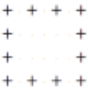
\includegraphics[width=2cm]{Cuadrado1.png}
    \end{figure}

    Cuando $m = 5$ ($m$ sea un numero impar)
    \begin{figure}[h]
        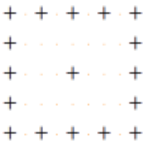
\includegraphics[width=3cm]{Cuadrado2.png}
    \end{figure}

    Donde $m$ es un número aleatorio entre 1 y 20, y cada número para imprime un cuadrado de base $m$ y cuando es impar de manera extra coloca el centro de la figura

    \hfil \break
    \textbf{Código}
    \begin{lstlisting}
codigo = false
    \end{lstlisting}

    \section*{Problema 2}
    Elabore un programa que reciba el del teclado un numero entero positivo mayor que 1, $k$ y realice un rombo cuya diagonal menor sea de tamaño $k$

    Ejemplo $k = 4$
    \begin{figure}[h]
        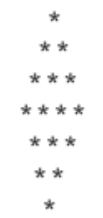
\includegraphics[width=2cm]{Rombo.png}
    \end{figure}

    \hfil \break
    \textbf{Código}
    \begin{lstlisting}
codigo = false
    \end{lstlisting}

    \section*{Problema 3}
    Realice un programa que reciba de entrada (de tipo Scanner) de 2 a 6 números enteros positivos y determinar quién es el menor, el de en medio y el mayor. Los números que se reciban serán de uno a uno, ósea de manera secuencial.

    Ejemplo, se la entrada $\longrightarrow 4 ,2, 9, 100, 89, 3$
    
    \hfil \break
    Salida:
    
    \hfil \break
    Mayor: 100 \\
    Menor: 2 \\
    Mediana: 4

    \hfil \break
    \textbf{Código}
    \begin{lstlisting}
codigo = false
    \end{lstlisting}

    \section*{Problema 4}
    Programar ``War of Numbers'' el ejercicio de describe en: \\
    \url{https://edabit.com/challenge/7fHsizQrTLXsPWMyH}

    Sólo que, en lugar de recibir un arreglo de enteros, la guerra sea con 10 números aleatorios entre 1-1000

    \hfil \break
    \textbf{Código}
    \begin{lstlisting}
codigo = false
    \end{lstlisting}

    \section*{Problema 5}
    Programar el problema descrito en: \\
    \url{https://edabit.com/challenge/4r33Yd2HuEireb3Sm}

    \hfil \break
    \textbf{Código}
    \begin{lstlisting}
codigo = false
    \end{lstlisting}
\end{document}